% 02.06.2016 12:00 CET last changed by a.holzinger
% General Template for LNCS and LNAI contributions based on llncs, adapted by ah
% Many thanks to the TRS team
% In case of using eps compile via 1) TeXify and then proceed with 2) dvi2pdf
%
\documentclass{llncs}
\usepackage{float}

\usepackage[dvips]{graphicx}
\usepackage[ruled,vlined]{algorithm2e}
\usepackage{amsfonts}
\usepackage{amssymb}
\usepackage{amsmath}
\usepackage{mathtools}

\providecommand{\abs}[1]{\lvert#1\rvert}
\providecommand{\norm}[1]{\lVert#1\rVert}

\usepackage{calc}
\usepackage{subfigure}

\usepackage{color}
\usepackage{soul}
\usepackage{comment}

\newtheorem{prop}{Property}

\newenvironment{Bitemize}{\renewcommand\labelitemi{\textbullet}\begin{itemize}}{\end{itemize}}

\begin{document}

\title{Interactive Anonymization\\
for Privacy aware Machine Learning}

\author{Bernd Malle\inst{1}\inst{2}, Peter Kieseberg\inst{1}\inst{2}, Andreas Holzinger\inst{1}}

\institute{Holzinger Group HCI-KDD \\
Institute for Medical Informatics, Statistics \& Documentation\\
            Medical University Graz, Austria\\
            \texttt{b.malle@hci-kdd.org}
\and
SBA Research gGmbH, Favoritenstraße 16, 1040 Wien \\
			\texttt{PKieseberg@sba-research.org}
}
	
\maketitle

% ==================================
%				ABSTRACT
% ==================================
\begin{abstract}

Privacy aware Machine Learning is the discipline of applying Machine Learning techniques in such a way as to ensure the privacy of people during the process. This can most easily achieved by first anonymizing a dataset before releasing it for the purpose of statistical data mining or research; starting in June 2018, this will also be the only legally permitted way within the European Union to release data without granting any people involved the 'right to be forgotten', i.e. the right to have their data deleted on request. To governments, organizations and corporations however, this represents a serious impediment to research operations, since any anonymization results in a certain degree of information loss and therefore reduced data utility. Our work focuses on applying interactive Machine Learning to the process of anonymization based on the idea of eliciting human background knowledge to optimize an algorithms parameters as to which attributes are more or less valuable to preserve. We demonstrate that human input can yield measurably better classification results than automatic approaches, with much more room for future improvement.


\medskip

\textbf{Keywords}: Machine Learning, Privacy aware ML, interactive ML, Knowledge Bases, Anonymization, k-Anonymity, SaNGreeA, Information Loss, Weight Vectors


\end{abstract}

\renewcommand{\thesubfigure}{\thefigure.\arabic{subfigure}}
\makeatletter
\renewcommand{\p@subfigure}{}
\renewcommand{\@thesubfigure}{\thesubfigure:\hskip\subfiglabelskip}
\makeatother


% ==================================
%			INTRODCUTION
% ==================================
\section{Introduction and Motivation}
\label{sect:intro_moti}

based on our initial PAML experiments \cite{}



% ==================================
%			  K-ANON
% ==================================
\section{k-anonymity (and beyond)}
\label{sect:k_anon}

Given the original tabular concept of anonymization, we will usually encounter three different categories of attributes within a given dataset:

\begin{itemize}
	\item \textbf{Personal identifiers} are data items which directly identify a person without having to cross-reference or further analyze them. Examples are email address or social security number (SSN). As personal identifiers are immediately dangerous, this category of data is usually removed.
	\item \textbf{Sensitive data,} also called 'payload', represents information that is crucial for further data mining or research purposes. Examples for this category would be disease classification, drug intake or personal income. This data shall be preserved in the anonymized dataset and can therefore not be deleted or generalized.
	\item \textbf{Quasi identifiers (QI's)}, are data which in themselves do not directly reveal the identity of a person, but might be used in aggregate to reconstruct it. For instance, \cite{sweeney2002k} reported in 2002 that the identity of 87\% of U.S. citizens could be uncovered via just the 3 attributes \textit{zip code}, \textit{gender} and \textit{date of birth}. Despite this danger, QI's may contain vital information to research applications (like ZIP code in a disease spread study); they are therefore generalized to an acceptable compromise between privacy (data loss) and information content (data utility).
\end{itemize}

Based on this categorization another formal concept of privacy was introduced as \textit{k-anonymity} \cite{Samarati:2001:kAnonymity}, in which a record is released only if its quasi-identifiers are indistinguishable from at least $k-1$ other entities in the dataset. This can be imagined like a clustering of data into so-called \textit{equivalence classes} of at least size $k$, with all internal QI's being generalized to the exact same level.

This original requirement of \textit{k-anonymity} \cite{Sweeney:2002:k-Anonymity} has since been extended by the concepts of \textit{l-diversity} \cite{MachanavajjhalaEtAl:2007:l-Diversity} (where every cluster must contain at least $l$ diverse sensitive values), \textit{t-closeness} \cite{LiEtAl:2007:t-closeness} (demanding that the local distribution over sensitive values must not diverge from its global distribution by more than a factor of $t$) as well as \textit{delta-presence} \cite{NergizClifton:2010:Delta-Presence} (which incorporates the background knowledge of a potential attacker). Although all of those concepts are interesting in their own right, for the sake of comparing interactive ML algorithms to  their fully automatic counterpart, we only took \textit{k-anonymity} into consideration (at least for this work).



% ==================================
%				iML
% ==================================
\section{interactive Machine Learning}
\label{sect:iML}

Interactive ML algorithms adjust their inner workings by continuously interacting with an outside \textit{oracle}, drawing positive / negative reinforcement from this interaction \cite{Holzinger:2016:iML}. Such systems are especially useful for highly-personalized predictions or decision support \cite{Kieseberg:2016:Doctor-in-the-Loop}; moreover many real-world problems exhibit (super)exponential algorithmic runtime; in such cases human brains dwarf machines at approximating solutions and learning from very small samples, thus enabling us to 'intuit' solutions efficiently \cite{iMLExperiment}.

By incorporating humans as oracles into this process, we can elicit background knowledge regarding specific use cases unknown to automatic algorithms \cite{WARE2001}. This however is highly dependent on the users' experience in a certain field as well as data / classification complexity; domain experts can of course be expected to contribute more valuable decision points than laymen; likewise, a low-dimensional dataset and simple classification tasks will result in higher quality human responses than convoluted problem sets.

While the authors of \cite{Moque2012} propose a system that interacts with a user in order to set a certain k-factor and subsequently provides a report on information loss and Kurtosis of QI distributions, the algorithm is not \textit{interactive} by our definition in that it does not influence the inner workings of the algorithm during the learning phase. This is also true in case of the Cornell Anonymization Toolkit (Cat) \cite{Xiao2009}, which conducts a complete anonymization run and only then lets the user decide if they are content with the results. In contrast, our approach alters algorithmic parameters upon every (batch of) human decisions, letting the algorithm adapt in real-time.

\cite{Loh2010} describe an approach incorporating humans into the anonymization process by allowing them to set constraints on attribute generalization; moreover they construct generalization hierarchies involving domain-specific ontologies. Although this technique marks a departure from wholesale automatic anonymization, it still lacks the dynamic human-computer interaction of our approach.

Apart from the field of privacy, interactive ML is today present in a wide spectrum of applications, from bordering medical fields like protein interactions / clusterings \cite{Amershi2014} via on-demand group-creation in social networks \cite{Amershi2012} to even teaching algorithms suitable mappings from gestures to music-generating parameters \cite{Fiebrink2009}.



% ==================================
%			EXPERIMENTS
% ==================================
\section{Experiments}
\label{sect:experiments}

The following sections will describe our experiment in detail, encompassing the general iML setting, the chosen  data set, anonymization algorithm used as well as a description of the overall pipeline employed to obtain the final results as presented.


\subsection{General setting}
\label{sect:setting}

The basic idea of our experiment was to compare different weight vectors representing attribute (quasi-identifier) importance during anonymization: Let's say that a doctor needs ro release a dataset for the purpose of studying disease-spread; in this case 'ZIP code' information is probably (but not necessarily) of much greater importance then 'occupation' or 'race'. However, if a skin cancer study is to be performed, 'race' information might be of utmost importance, whereas 'ZIP code' might be negligible.

In our experiment, the task was to classify a people dataset on the target attributes \textit{income}, \textit{education level} and \textit{marital status}. Therefore, we tested an \textit{equal} weight vector setting against two others obtained from human experiments: 1) \textit{bias} in which the user just specified which attributes they thought would be important for a specific classification by moving sliders, and 2) \textit{iML} in which the user was tasked to decide a series of clustering possibilities by moving a data row to one of two partly anonymized clusters presented, thereby conveying which attributes were more important to preserve than others Figure~\ref{fig:iml_UI}.

\begin{figure}[!h]
	\begin{center}
		\vspace{-1.0cm}
		\hspace*{-0.8cm}
		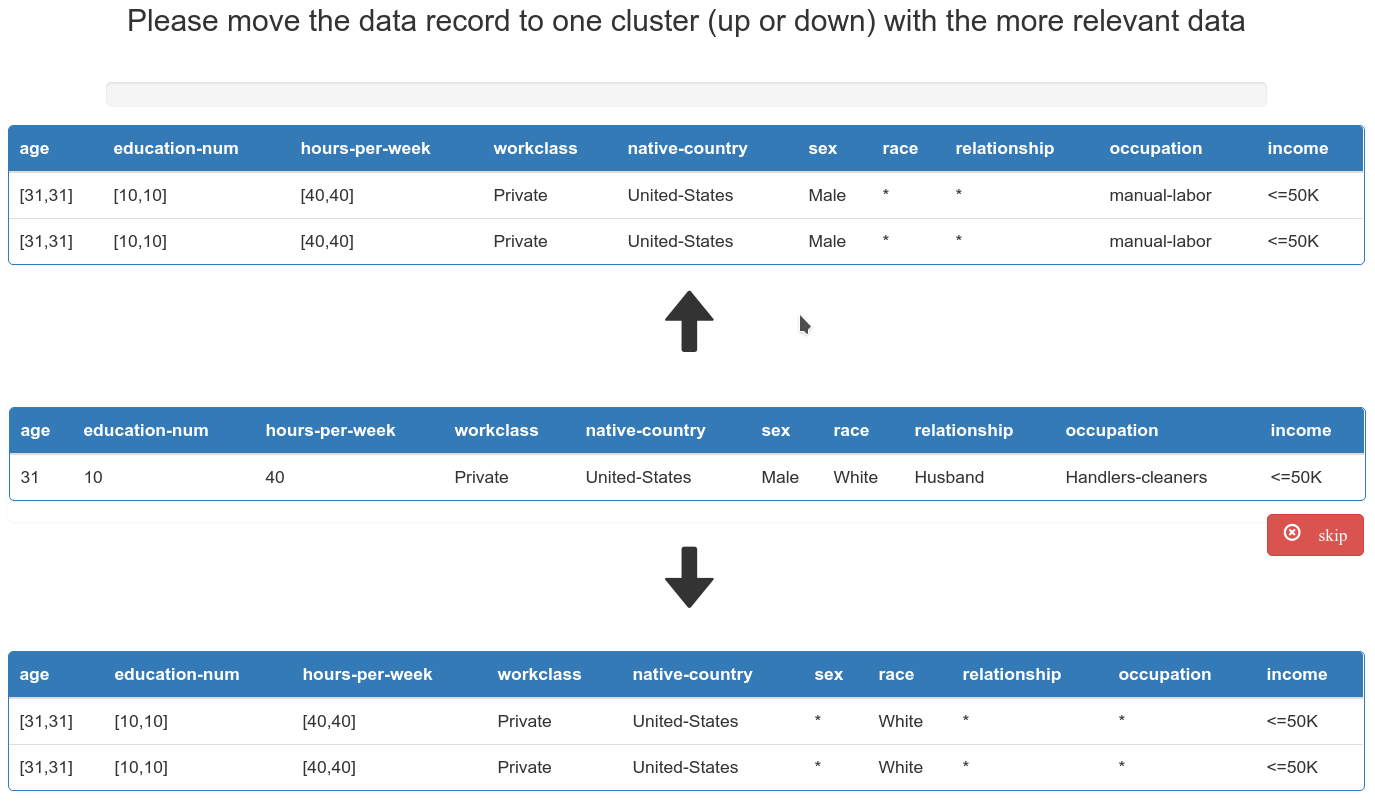
\includegraphics[width=1.0\textwidth]{figures/iml_anon_screen1}
		
		\vspace{1.0cm}
		\hspace*{-0.8cm}
		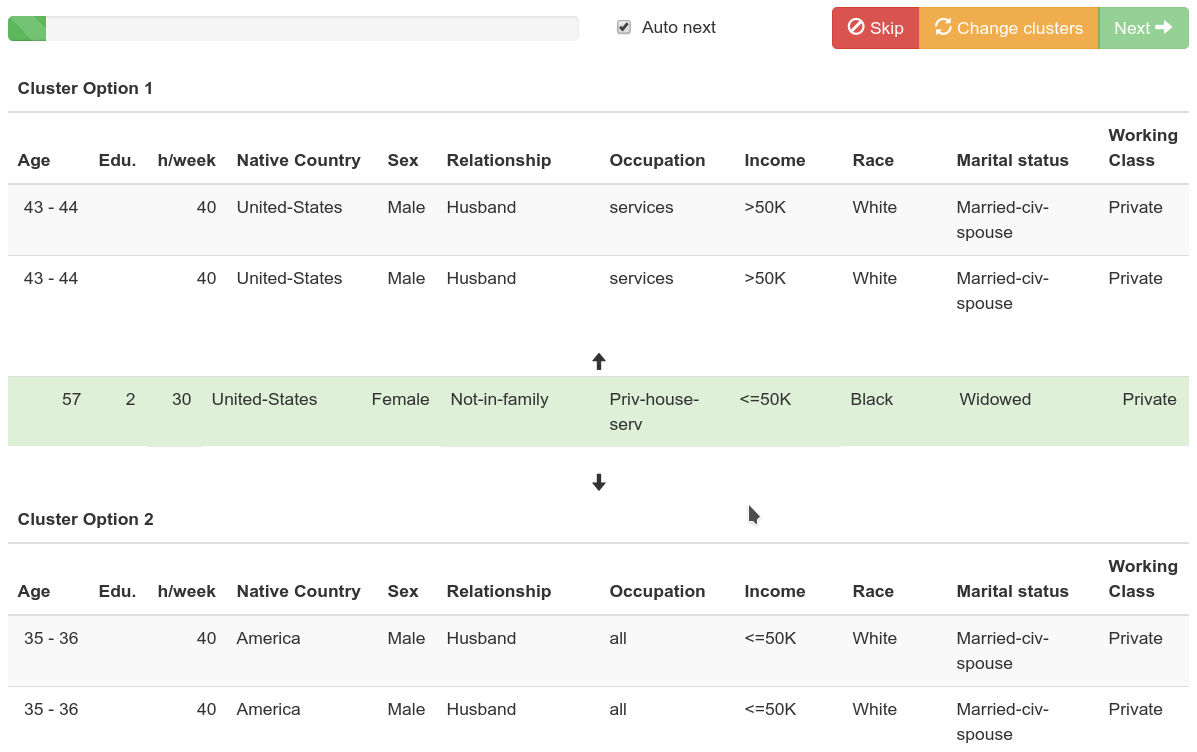
\includegraphics[width=1.0\textwidth]{figures/iml_anon_screen2}
		\caption{Two different implementations of the iML interface design.}
		\label{fig:iml_UI}
	\end{center}
\end{figure}


\subsection{Data} 
\label{ssect:data}

We chose the adults dataset from the UCI Machine Learning repository which was generated from US census data from 1994 and contains approximately 50k entries in it's original; after initial preprocessing we chose the first 500 complete data rows as our iML experimental data to be presented to users via a Web Browser UI. After obtaining bias / iml weights from the experiment, we chose the first 3k entries of the original data as the basis for producing 780 new, anonymized data sets. Although this might seem overly frugal on our part, we have asserted via random deletion of original data points that classifier performance remains stable for as little as 1.5k randomly selected rows. 
Of the original attributes (data columns) provided 4 were deleted: 'capital-gain' \& 'capital-loss' (both were too skewed to be useful for humans), 'fnlwgt' (a mere weighting factor) as well as 'education' which was also represented by a column containing its numerical mapping ('education\_num').


\subsection{Algorithm}
\label{ssect:algorithm}

In order to conduct our experiments, it was necessary to choose an algorithm which would enable us to easily hook into its internal logic - we therefore chose a greedy clustering algorithm called \textit{SaNGreeA} (Social network greedy clustering) which was introduced by \cite{campan2009data} and implemented it in JavaScript. This enabled us to execute it within a browser environment during our iML experiments as well as server-side for batch-execution of all derived datasets later on.

Besides its capacity to anonymize graph structures (which we did not utilize during this work), it is a relatively simple algorithm considering \textit{General information loss} - or GIL - during anonymization. This GIL can be interpreted by the sum of information loss occurring during generalization of continuous (range) as well as hierarchical attributes:

\begin{equation*}
\begin{split}
\text{GIL}(cl) = \abs{cl} \cdot (\sum_{j=1}^{s} \frac{size(gen(cl)[N_j])}{size(min_{x \epsilon N} (X[N_j]), max_{x \epsilon N} (X[N_j]))} \\
+ \sum_{j=1}^{t} \frac{height(\Lambda(gen(cl)[C_j]))}{height(H_{C_j})})
\end{split}
\end{equation*}


where:\\
- $\abs{cl}$ denotes the cluster cl's cardinality; \\
- $size([i1,i2])$ is the size of the interval $[i1,i2]$, i.e., $(i2-i1)$; \\
- $\Lambda(w), w \epsilon H_{C_j}$ is the sub-hierarchy of $H_{C_j}$ rooted in $w$; \\
- $height(H_{C_j})$ denotes the height of the tree hierarchy $H_{C_j}$; \\


The total generalization information loss is then given by:
\begin{equation*}
\text{GIL}(G,S) = \sum_{j=1}^{v} \text{GIL}(cl_j)
\end{equation*}
And the normalized generalization information loss by:
\begin{equation*}
\text{NGIL}(G,S) = \frac{\text{GIL}(G,S)}{n \cdot (s+t)}
\end{equation*}

The algorithm starts by picking a (random or pre-defined) data row as its first cluster, then iteratively picking best candidates for merging by minimizing GIL until the cluster reaches size $k$, at which point a new data point is chosen as the initiator for the next cluster; this process continues until all data points are merged into clusters, satisfying the $k$-anonymity criterion for the given dataset.


\subsection{Processing pipeline for obtaining results}
\label{ssect:process}

Once our iML experiments had yielded enough weight vectors, we had to generate a whole new set of anonymized datasets on which we subsequently applied 4 classifiers on each of the 3 target attributes (columns) described; therefore we designed the following processing pipeline:


\begin{enumerate}
	\item Taking the first 5k rows of the original, preprocessed dataset as input and applying k-anonymization with a k-factor range of [5, 10, 20, 50, 100, 200] and 129 different weight vectors (equal, bias, iml) from our experiments on it, we produced 774 anonymized datasets (775 including the original).
	%\item We then ran 4 different classifiers on it and computed precision, recall as well as F1 score. The four classifiers used were \textit{gradient boosting}, \textit{random forest}, \textit{logistic regression} and \textit{linear SVC}.
	%\item From the obtained results we extracted the 3 attribute values most contributing to a "positive" ($>$50k) result as well as the top 3 attribute values indicating a "negative" ($<=$50k) prediction as depicted in Figure~\ref{fig:adult_important_columns}
	%\item For each of these 6 attribute values, we subsequently deleted a specific percentage of data rows containing that value from the original dataset, resulting in 30 reduced datasets. The 5 percentages used were $0.2$, $0.4$, $0.6$, $0.8$ as well as $1.0$.
	%\item To each of those datasets we re-applied the four chosen classifiers successively and recorded the respective impact on the quality of the classification result. The results can be seen in Figure~\ref{fig:adult_results_perturbation_top} and Figure~\ref{fig:adult_results_perturbation_bottom}.
	%\item In order to measure the effects of k-anonymization on classifier performance, we used the SaNGreeA's GIL component described in the following section to generate datasets with a k-factor of $k=3$, $k=7$, $k=11$, $k=15$ as well as $k=19$. Furthermore, we used each of these settings with 3 different weight vectors: 1) equal weights for all attributes, 2) age information preferred ($\omega(age)=0.88$, $\omega(other\_attributes)=0.01$) and 3) race information preferred ($\omega(race)=0.88$, $\omega(other\_attributes)=0.01$). We then re-executed all classifiers on the resulting 15 datasets and recorded the respective results, which can be seen in Figure~\ref{fig:adult_results_anonymization}.
\end{enumerate}


% ==================================
%		RESULTS & DISCUSSION
% ==================================
\section{Results \& Discussion}
\label{sect:results}

\begin{figure}[!h]
	\begin{center}
		\vspace{-1.0cm}
		\hspace*{-0.8cm}
		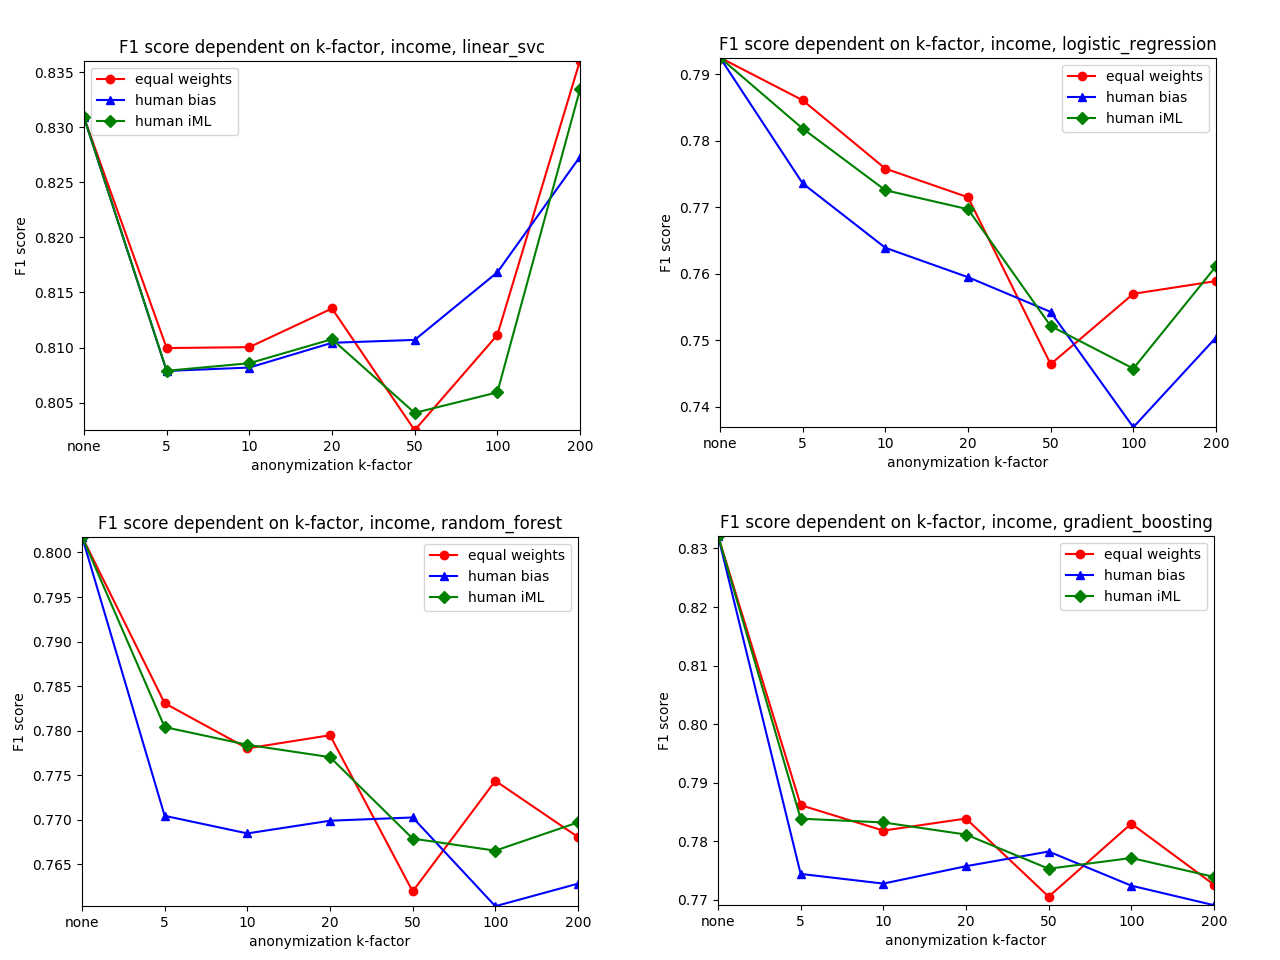
\includegraphics[width=1.0\textwidth]{figures/income.png}
		\caption{Results on...}
		\label{fig:results_income}
	\end{center}
\end{figure}

\begin{figure}[!h]
	\begin{center}
		\vspace{-1.0cm}
		\hspace*{-0.8cm}
		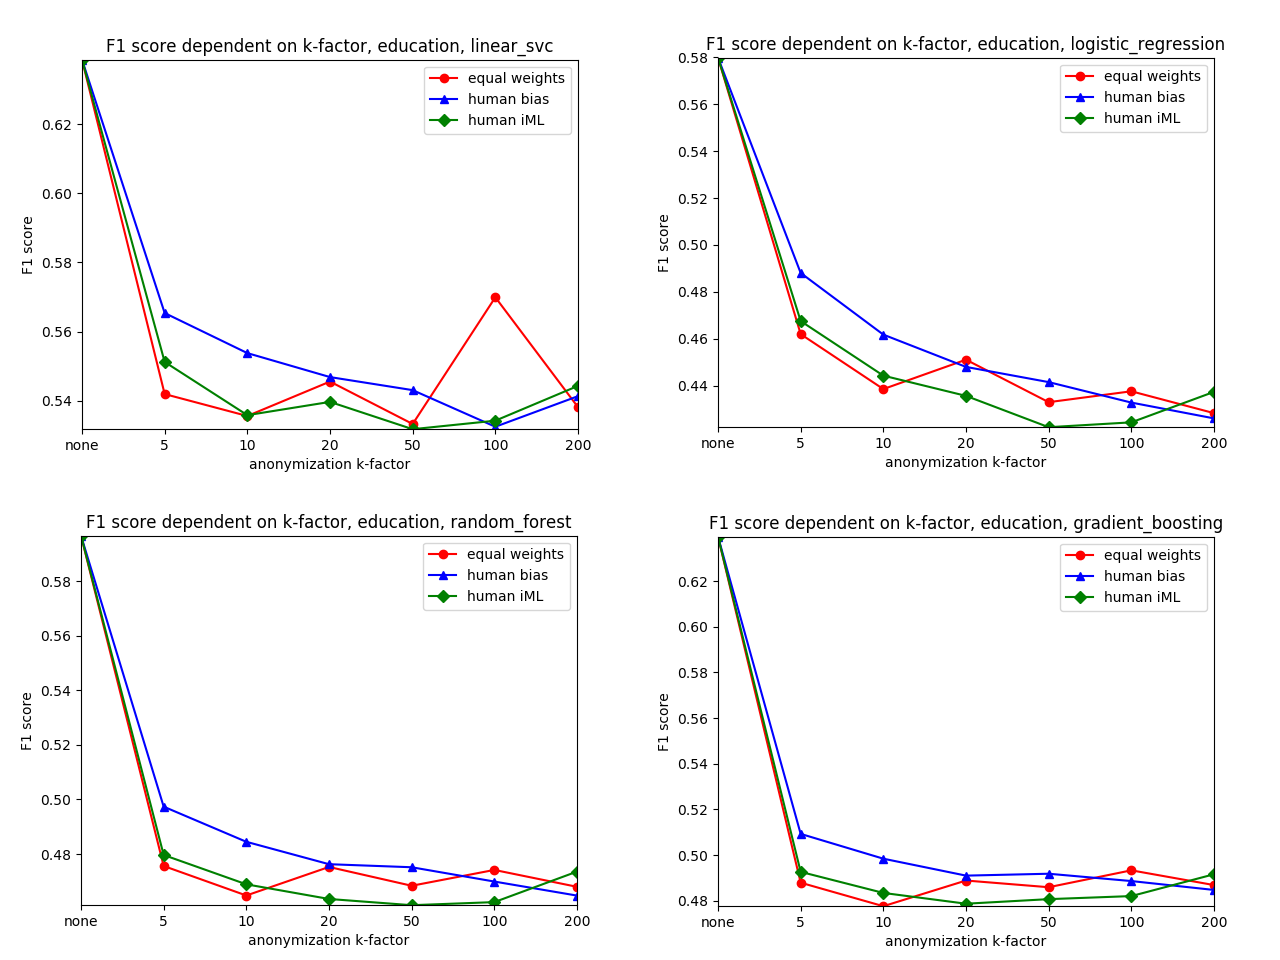
\includegraphics[width=1.0\textwidth]{figures/education_num.png}
		\caption{Results on...}
		\label{fig:results_education}
	\end{center}
\end{figure}

\begin{figure}[!h]
	\begin{center}
		\vspace{-1.0cm}
		\hspace*{-0.8cm}
		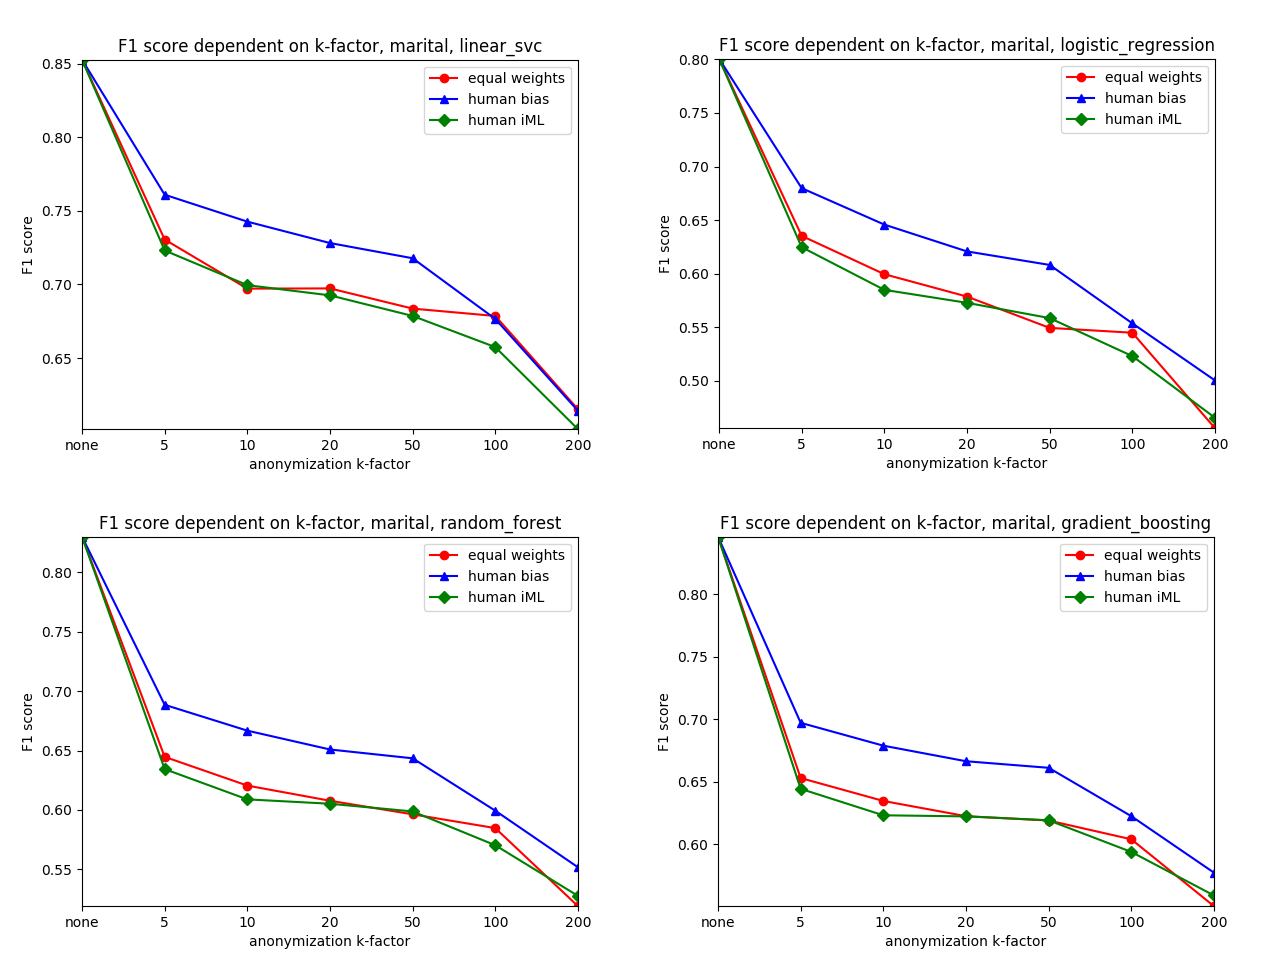
\includegraphics[width=1.0\textwidth]{figures/marital_status.png}
		\caption{Results on...}
		\label{fig:results_marital}
	\end{center}
\end{figure}



% ==================================
%		PROBLEMS & CHALLENGES
% ==================================
\section{Open problems \& future challenges}
\label{sect:op_fc}

\begin{itemize}
	\item \textbf{Explain the unexpected behavior} for...
\end{itemize}


% ==================================
%			CONCLUSION
% ==================================
\section{Conclusion}
\label{sect:conclusion}


\clearpage
\newpage

\bibliographystyle{plain}
\bibliography{references}

\end{document}

